\chapter{Marco teórico}
\label{capitulo1}
\lhead{Capítulo 1. \emph{Marco teórico}}

\section{Descubrimiento de Conocimiento y preprocesamiento de datos}

Hoy en día existe una creciente necesidad de procesar grandes volúmenes de datos, estos datos son producto de la recolección de información de procesos y actividades de distintas índoles y se vuelven un material valioso para extraer información sobre posibles tendencias que puedan existir en dichos procesos \cite{han2011data}. Es aquí donde entra el \emph{Descubrimiento de Conocimiento en Bases de Datos} (KDD por su siglas en inglés) como disciplina encargada del procesamiento de datos para la extracción de información.

KDD es definida por \emph{Smyth, P. et al.} \cite{fayyd1996data} como ``el proceso no trivial de identificar patrones en los datos que sean válidos, novedosos, potencialmente útiles y finalmente entendibles''. Para este fin, KDD se subdivide en distintas etapas a llevar a cabo para lograr el fin último de identificar patrones, éstas son \cite{garcia2016data}: especificación del problema, entendimiento del problema, preprocesamiento de los datos, minería de datos, evaluación de los resultados y explotación de los resultados. En el presente trabajo de investigación es de especial interés la etapa de preprocesamiento de datos.

El preprocesamiento de datos consiste en el conjunto actividades destinadas a preparar los datos para ser usado por un Algoritmo de Minería de Datos (DM por sus siglas en inglés). Las actividades realizadas en el preprocesamiento pueden ser clasificadas como actividades para la preparación de los datos y la reducción de los mismos \cite{garcia2016data}.

La preparación de datos es un paso obligatorio en el preprocesamiento, ya que transforma los datos, que inicialmente no se pueden utilizar con el algoritmo de DM por asuntos como la presencia de atributos faltantes en instancias, datos erróneos y atributos con formatos no aceptables para el algoritmo a utilizar \cite{garcia2016data}. Dependiendo del enfoque dado, estas actividades pueden clasificarse en los siguientes parámetros:

\begin{itemize}
\item \textbf{Limpieza de datos \cite{garcia2016data, kim2003taxonomy}:}
incluye el tratamiento de los atributos faltantes y los datos erróneos, que si se dejan sin tratar resulta en un modelo de minería de datos poco confiable. Un atributo faltante en una instancia ocurre como consecuencia de no haberse introducido al momento del registro o bien por la pérdida en el proceso de almacenamiento. Los datos con atributos faltantes pueden tratarse de tres maneras \cite{farhangfar2007novel}: la eliminación de las instancias que presenten el problema, utilizar métodos de estimación de máxima verosimilitud para calcular promedios y varianzas y utilizar algoritmos del repertorio de \emph{machine learning} como k-nn, k-means o  \emph{Suport Vector Machine} para estimar el valor de los atributos faltantes. 

Por su parte, los datos erróneos (también conocidos como ``datos ruidosos'') pueden venir de dos formas \cite{catal2011class}: se llama ``ruido de clase'' cuando la instancia está mal clasificada y ``ruido de atributo'' cuando uno o más valores de los atributos en una instancia están distorsionados y no representan la realidad. Para tratar los datos ruidosos se pueden usar tres métodos: construir algoritmos de DM que no se vean afectados en cierta medida ante el ruido (sean robustos), pulir los datos \cite{teng1999correcting} de tal manera que se corrijan los errores y por último se puede identificar los datos ruidosos para eliminarlos del conjunto y así quedarse sólo con datos correctos \cite{brodley1999identifying}.

\item \textbf{Transformación de datos \cite{garcia2016data}:}
se centra en aplicar fórmulas matemáticas a los valores de los atributos para así obtener valores sintéticos que puedan proporcionar más información respecto a la instancia y al conjunto que pertenecen, las transformaciones más comunes son la lineal y la cuadrática.

\item \textbf{Integración de los datos \cite{garcia2016data,batini1986comparative}:}
consiste en la unión de los conjuntos de datos provenientes de distintas fuentes en un único conjunto. La integración tiene que tomar en cuenta algunos aspectos que se pueden presentar durante el proceso, entre ellos están la redundacia de atributos, la cual sucede cuando dos atributos están fuertemente correlacionados. La redundancia de atributos puede traer consigo un \emph{sobre ajuste} (\emph{overfitting} en inglés) de los modelos predictivos, además de aumentar el tiempo de cómputo de los mismos, es por eso que se debe eliminar la redundancia y para ello se utiliza una prueba de correlación $\chi^2$ con el fin de identificar los atributos redundantes y así decidir con cual quedarse. 

Al continuar con los problemas que se pueden presentar al momento de la integración, se tiene también la duplicación de instancias, problema que normalmente trae consigo la inconsistencia en los valores de los atributos, debido a las diferencias con las que se registran los valores. Para solucionar este asunto, primero se tiene que identificar las instancias duplicadas usando técnicas que midan la similitud entre ellas, como la propuesta de \emph{Fellegi, I. \& Sunter, A.} \cite{fellegi1969theory} que lo modela como un problema de inferencia bayesiana o como en \cite{cochinwala2001efficient} donde se usan árboles de clasificación y regresión (CART por sus siglas en inglés) para cumplir este trabajo.

\item \textbf{Normalización de datos \cite{garcia2016data}:}
busca cambiar la distribución de los datos originales de tal manera que se acoplen a las necesidades de los algoritmos predictivos. Dos de los tipos de normalización más usadas son la normalización min-max y la normalización \emph{z-score}.

\end{itemize}

A pasar a la reducción de los datos, se tiene que engloba todas las técnicas que reducen el conjunto de datos original para obtener uno representativo con el cual trabajar en los modelos predictivos. La reducción de datos cobra especial importancia cuando se tienen conjuntos muy grandes que tienden a elevar en gran medida el tiempo de cómputo de los algoritmos que los van a usar. Las técnicas de reducción de datos son \cite{garcia2016data}:

\begin{itemize}
\item \textbf{Discretización de datos \cite{garcia2016data,garcia2013survey}:}
es el proceso de transformar datos numéricos en datos categóricos, al definir un número finito de intervalos que representan rangos entre distintos valores consecutivos con el fin de poder tratarlos como valores nominales. Es de especial importancia conseguir el número correcto de intervalos que mantengan la información original de los datos, ya que muy pocos intervalos puede llegar a ocultar la relación existente entre un rango en específico y una clase dada y muchos intervalos puede llevar a un sobre ajuste \cite{cios2007data}. El principal atractivo de la discretización es que permite utilizar un algoritmo de DM que trabaje principalmente con datos nominales como \emph{Naïve Bayes} \cite{yang2009discretization} a partir de datos numéricos. Para un estudio más completo de la discretización se referencia a \cite{garcia2013survey}.

\item \textbf{Selección de características \cite{garcia2016data,liu2012feature}:}
busca eliminar atributos que sean redundantes o irrelevantes de tal manera que el subconjunto de características restantes mantenga la distribución original de las clases. El proceso de selección de características tiene ventajas, como mantener e incluso mejorar la precisión de los modelos predictivos, reducir los tiempos de cómputo y reducir la complejidad de los modelos resultantes. La búsqueda de un subconjunto de atributos puede realizarse de tres maneras: búsqueda exhaustiva, búsqueda heurística y métodos no determinísticos. La búsqueda exhaustiva cubre todo el espacio de soluciones, normalmente prueban todas las combinaciones posibles de atributos para conseguir el que mejor se acople a la métrica a optimizar, entre los métodos exhaustivos están \emph{Focus} \cite{almuallim1991learning}, \emph{Automatic Branch \& Bound} \cite{liul1998monotonic}, \emph{Best First Search} \cite{xu1988best}, entre otros. Por su parte, la búsqueda heurística encuentra una solución aproximada a la óptima en poco tiempo, entre sus métodos están los propuestos en \cite{dash1997feature,koller1996toward,battiti1994using}. Por último, están los métodos no determinísticos, de entre los que destacan las metaheurísticas evolutivas, recocido simulado y \emph{Las Vegas Filter} \cite{liu1996probabilistic}.

\item \textbf{Selección de instancias \cite{garcia2016data}:}
consiste en elegir un subconjunto de las instancias totales que mantengan las características del conjunto original. Este es el problema desarrollado en esta investigación y se elabora más sobre el mismo en la siguiente sección.
\end{itemize}

\section{Selección de Instancias y Selección de Prototipos}

La Selección de Instancias (IS por sus siglas en inglés) consiste en reducir el conjunto de datos dado a un conjunto reducido que conserve las capacidades de representación del conjunto original, para ser utilizado con un algoritmo de clasificación o regresión, que mantenga el desempeño del algoritmo como si se usara el conjunto original.\\

\begin{definicion}
Dado un conjunto de datos X, se tiene que una instancia $X_i = (X_i^1,X_i^2,\dots,X_i^p)$ donde $X_i^j$ es el atributo $j$ para la instancia $X_i$ con $X_i\in X$ y $p$ es el número de atributos. La instancia $X_i$ es de clase $Y_j$ donde $Y_j\in Y$, Y es el conjunto de todas las clases definidas con $j\in (1\dots q)$ donde $q$ es el número de clases totales. A continuación, se divide el conjunto $X$ en un conjunto $TR$ de entrenamiento y un conjunto $TS$ de prueba. El problema de \textbf{Selección de Instancias} consiste en conseguir un conjunto reducido $S\subseteq TR$ con el cual, al usarse con el clasificador M se mantenga o mejore la capacidad de representación del conjunto original \cite{garcia2016data}.
\end{definicion}

La respuesta óptima de un método de selección de instancias es un conjunto \emph{consistente} y de cardinalidad mínima.\\

\begin{definicion}
Un conjunto $R$ es \textbf{consistente} con $T$, \emph{si y solo si} toda instancia $t \in T$ es clasificada correctamente mediante el uso de un clasificador \emph{M} y las instancias en $R$ como conjunto de entrenamiento. \cite{flores2014metaheuristics}
\end{definicion}

Sin embargo, conseguir la respuesta óptima es un problema NP-Duro (\emph{NP-Hard}) como lo demuestra \emph{Zukhba, A.} en \cite{zukhba2010np}. Por lo tanto, la mayoría de los métodos propuestos hasta la fecha se enfocan en obtener una solución aproximada.

El problema de selección de instancias se puede enfocar como un problema de selección de prototipos (PS por sus siglas en inglés). PS es en esencia IS con el detalle de que el clasificador M usado es un clasificador ``1 Vecino Más Cercano'' (1-NN por sus siglas en inglés) \cite{garcia2016data}.

%\subsection{Regla de K vecinos más cercanos}

%Inicialmente propuesta por \emph{Fix, E. \& Hodges, J.} en \cite{fix1951discriminatory}. La regla KNN clasifica instancias a partir de los datos adyacentes; esto viene dado bajo el razonamiento de que una instancia probablemente comparta la misma clase que sus vecinos. Formalmente, el algoritmo de clasificación usando KNN se puede definir como:\\  

%\begin{definicion}
%Sea X un conjunto de datos con $X_i\in X$ una instancia del conjunto, con clase $Y_{X_i}\in Y$ la clase a la cual pertenece, siendo Y el conjunto de las clases presentes en los datos. Sea $\pi_1(X_i)\dots \pi_n(X_i)$ un reordenamiento de las n instancias que conforman el conjunto X de acuerdo a la distancia a la que se encuentren de la instancia $X_i$, usando una métrica de distancia dada $\rho:\chi$ \texttt{X} $\chi \rightarrow \mathbb{R}$, donde $\chi$ es el dominio de las instancias en X, tal que $\rho(X_i,\pi_k(X_i)) \leq \rho(X_i,\pi_{k+1}(X_i))$. Para clasificar una instancia $X_j$ se usa la clase de la mayoría perteneciente al conjunto $\left\{Y_{\pi_i(X_j)} \mid i \leq k\right\}$ siendo k el número de vecinos que se toma en consideración. \cite{shalev2014understanding}
%\end{definicion}

%Lo simple del algoritmo ha impulsado KNN a ser uno de los algoritmos de DM más usados y ha inspirado numerosos estudios sobre el comportamiento de convergencia y acotaciones sobre el error en la clasificación. Entre dichos trabajos se encuentra el de \emph{Cover, T. \& Hart, P.} \cite{cover1967nearest} donde muestran que la probabilidad de error R del clasificador NN está acotada por debajo por la probabilidad de error de Bayes R* y acotada por arriba por $R^*(\frac{2-MR^*}{M-1})$ cuando el número de instancias tiende al infinito y además la regla NN es admisible en la clase de reglas KNN, esto quiere decir que no hay $k\neq 1$ para el cual la probabilidad de error R sea menor que para $k=1$. Para un estudio más formal de las propiedades de convergencia se refiere a \cite{devroye2013probabilistic}.

%Una implementación ingenua de KNN dado una instancia a clasificar q, consta de calcular la distancia de todos los puntos con respecto a q y reportar los k puntos más cercanos; esto tiene una complejidad de $O(dn)$ donde d es el número de atributos en una instancia y n es el total de instancias \cite{shakhnarovich2006nearest}. Es por eso que mucho de los esfuerzos de la investigación de KNN es encontrar estructuras de ordenado y almacenamiento que lleven la complejidad a un orden sublineal o inclusive logarítmico; entre ellas están:

%\begin{itemize}
%\item \textbf{Árboles KD \cite{shakhnarovich2006nearest,bentley1975multidimensional}:}
%también conocidos como \emph{KD Trees} en inglés, se construyen de la siguiente manera: dado n puntos en un conjunto P en un espacio d-dimensional, primero se calcula la mediana M de los valores del i-ésimo atributo de los n puntos (inicialmente i = 1) y con este valor M se particiona el conjunto P en $P_L$ como el conjunto con puntos cuyo valor del i-ésimo atributo es menor a M y $P_R$ como el conjunto de puntos cuyo valor del i-ésimo atributo es mayor o igual a M. En la siguiente iteración se elige otro atributo i y se particionan $P_L$ y $P_R$ en dos cada uno. El proceso se repite hasta que el conjunto de puntos en un nodo del árbol construido llegue a tener cardinalidad 1. El tiempo de construcción del árbol es de O(nlog(n)) y el tiempo de búsqueda en G(d)log(n) dado una función G la cual es exponencial en d, cabe destacar que el tiempo de búsqueda es al lo sumo O(dn).

%\item \textbf{Árboles de esfera \cite{shakhnarovich2006nearest,omohundro1989five,uhlmann1991satisfying}:}
%los árboles de esfera (\emph{balltrees} en inglés) son árboles binarios donde las hojas corresponden a las instancias y cada nodo interior del árbol corresponde a una esfera en el espacio de los datos, cada esfera requiere ser la más pequeña que contenga las esferas asociadas a los nodos hijos. En contraste con los árboles KD, las regiones asociadas entre nodos vecinos en los árboles de esfera pueden intersectarse y no tienen que cubrir la totalidad del espacio, lo que permite una cobertura más flexible que refleje la estructura inherente a los datos.

%\item \textbf{Hashing sensitivo a la localidad \cite{shakhnarovich2006nearest,indyk2004nearest}:}
%la idea principal detrás del Hashing Sensitivo a la localidad (LSH por sus siglas en inglés) es realizar un hashing con los datos usando varias funciones de hash de tal manera que la probabilidad de colisión entre dos puntos sea mayor mientras más cerca estén uno del otro usando una métrica de distancia. Entonces, una vez construida la tabla de hash, se puede determinar los vecinos más cercanos retornando los elementos en el contenedor correspondiente a su valor calculado por la función de hash.
%\end{itemize}

%Un concepto que está presente al momento de clasificar usando KNN es la llamada maldición de dimensionalidad, ésta afecta la clasificación de dos maneras: la primera estipula que un pequeño incremento en las dimensiones de los datos trae consigo un gran aumento en el número de instancias necesarias para mantener la misma precisión del clasificador. La segunda, por su parte, menciona que para métodos de almacenamiento como los árboles KD y los árboles esfera un aumento en las dimensiones tiende a degradar su desempeño a una búsqueda lineal como la implementación ingenua \cite{keogh2017curse}. Lo cual afecta la aplicabilidad del algoritmo a datos de muy grandes dimensiones y abre un campo de estudio continuo a formas de optimización del ordenamiento y almacenamiento de las instancias.

\subsection{Taxonomía del problema de selección de prototipos}

En la presente investigación se toman las propuestas taxonómicas de \emph{García, S. et al.} en \cite{garcia2012prototype}. Este procedimiento de clasificación permite agrupar los métodos según distintos criterios: si el método de selección parte de un conjunto vacío o del conjunto original; si usan un esquema de validación cruzada o no o si las instancias preservadas son las más cercanas a los límites entre clases o son las instancias centrales. Esta taxonomía se utiliza para hacer la elección de las heurísticas a utilzar, de tal manera que sean distintas entre sí y así poder estudiar los diferentes comportamientos al combinarlas con metaheurísticas.


\subsubsection{Dirección de búsqueda}

\begin{itemize}
\item \textbf{Incremental:}
se empieza con un conjunto vacío S y se añaden instancias de TR si cumple con cierto criterio. El orden de presentación de las instancias puede llegar a afectar el resultado final para muchos algoritmos, por eso se acostumbra a presentar los datos de manera aleatoria. Una búsqueda incremental tiene la ventaja de que se pueden agregar instancias una vez finalizado un proceso de selección inicial, aspecto característico lo hace bastante atractivo para el aprendizaje continuo

\item \textbf{Decremental:}
la búsqueda empieza con S = TR y se seleccionan instancias para remover de S. El orden de presentación todavía es importante, pero a diferencia de los métodos incrementales, se tiene todo el conjunto desde el inicio. Los algoritmos decrementales tienden a presentar un mayor costo computacional que los incrementales.

\item \textbf{Por lote:}
se elige un grupo y se evalúan todos los elementos del mismo para su eliminación, los que no pasen la prueba seleccionada son desechados. El proceso se repite con distintos lotes hasta terminar.

\item \textbf{Mixto:}
S empieza como un subconjunto preseleccionado (puede ser de manera aleatoria o usando un proceso incremental/decremental) e iterativamente puede añadir o remover instancias que cumplan con criterios en específico.

\item \textbf{Fijo:}
el número final de instancias en S se fija al principio de la fase de aprendizaje y se aplica una búsqueda mixta hasta cumplir con dicha cuota.
\end{itemize}

\subsubsection{Tipo de selección}

\begin{itemize}
\item \textbf{Condensación:}
se busca mantener los puntos bordes (aquellos que están cercas de las fronteras entre las clases). El razonamiento es que son los puntos bordes los que realmente determinan las fronteras, ya que son más útiles al momento de clasificar una nueva instancia. Estos métodos tienden a reducir bastante el conjunto original ya que hay menos puntos bordes que interiores.

\item \textbf{Edición:}
los métodos de edición en cambio buscan remover los puntos bordes, con lo que se suavizan las fronteras bajo la idea de que es el lugar donde se concentran la mayor cantidad de puntos ruidosos. Tienden a disminuir en menor medida el conjunto TR en comparación a los métodos de condensación.

\item \textbf{Híbridos:}
su principal objetivo es mantener la precisión del clasificador al usar un conjunto lo más reducido posible. Para esto eliminan tanto puntos internos como los ruidosos en el borde, al tomar las ideas principales de los métodos de condensación y edición.
\end{itemize}

\subsubsection{Evaluación de la búsqueda}

\begin{itemize}
\item \textbf{Filtro:}
son los métodos que no usan esquema de validación cruzada (se explica este esquema en el siguiente capítulo). Se caracterizan por conseguir resultados rápidamente. 

\item \textbf{Envolventes:}
usan todo el conjunto TR en un proceso de validación cruzada. Son métodos más costosos que los filtros, pero tienden a obtener una precisión mayor al momento de generalizar al usar un algoritmo de DM.
\end{itemize}

A continuación se presenta en la la figura \ref{taxonomia} la clasificación que se le puede dar a los algoritmos. Para un estudio más extenso sobre los distintos algoritmos se recomienda leer \cite{garcia2016data}

\begin{figure}[]
\centering
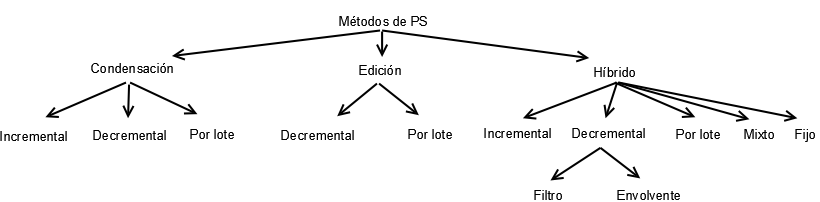
\includegraphics[width=\textwidth]{taxonomia.png}
\caption[Taxonomía para los métodos de selección de prototipos]{Taxonomía para los métodos de selección de prototipos}
\label{taxonomia}
\end{figure}

\subsection{Heurísticas}

En esta sección se exponen las heurísticas utilizadas en este trabajo. De acuerdo con \emph{Pearl, J.} en \cite{pearl1984heuristics}: ``Una heurística es un criterio, método o principio para decidir cual, de entre varias alternativas de acciones a seguir, promete ser la más efectiva para alcanzar un objetivo''. Para el caso de PS, dicho objetivo es alcanzar un buen aproximado al conjunto de cardinalidad mínima y máxima precisión en la clasificación.

\subsubsection{Condensed Nearest Neighbor (CNN)}

Propuesto inicialmente por \emph{Hart, P.} en \cite{hart1968condensed},CNN es un método de condensación incremental. El conjunto S se construye de tal manera que cada elemento de TR está más cerca de un miembro de S de la misma clase que un miembro de S de clase distinta. El algoritmo empiza con la selección de una instancia aleatoria $s$ y se coloca en $S$ (inicialmente vacío), acto seguido se empieza a clasificar las instancias de TR sólo usando las instancias pertenecientes $S$; si una instancia es clasificada incorrectamente, se agrega a $S$, lo que asegura así que en la siguiente vuelta sea clasificada correctamente. Una vez aumentado $S$ se vuelve a probar cada instancia de TR y se agregan las que sean mal clasificadas. El proceso se repite hasta que no existan instancias en TR que se encuentren mal clasificadas. CNN se presenta en el algoritmo \ref{cnn}. 

\begin{algorithm}
\caption{CNN}
\label{cnn}
\begin{algorithmic}[1]

\Require $TR$ conjunto de entrenamiento
\Ensure Conjunto reducido $S$, $S \subseteq TR$

\State $S \gets \left\lbrace \mathrm{Una\ instancia\ cualquiera}\ t \in TR \right\rbrace$
\Repeat
	\State $S' \gets S$
	\ForAll{$t \in TR$}
		\If{$t$ es mal clasificada usando $S$ con un clasificador 1-NN}
			\State $S \gets S \cup \left\lbrace t \right\rbrace$
		\EndIf
	\EndFor
\Until{$S = S'$}
\State \Return{$S$}
\end{algorithmic}
\end{algorithm}


\subsubsection{Edited Nearest Neighbor (ENN)}

Propuesto por  \emph{Wilson, D.} en \cite{wilson1972asymptotic}, ENN es un método de edición decremental. Empieza con S = TR y se itera sobre las instancias de S, de modo que se remueven aquellas que no concuerdan con la clase de su vecino más cercano. ENN se presenta en el algoritmo \ref{enn}.

\begin{algorithm}
\caption{ENN}
\label{enn}
\begin{algorithmic}[1]

\Require{\texttt{TR} conjunto de entrenamiento}
\Ensure{\texttt{S} conjunto reducido}

\State $S \gets$ TR
\For{$s \in S$}
  \If{la clase de $s$ es distinta a la clase de su vecino más cercano}
    \State Se elimina s de S
  \EndIf
\EndFor

\State \Return S

\end{algorithmic}
\end{algorithm}

\subsubsection{Relaxed Selective Subset (RSS)}

 Al observar la propuesta de \emph{Flores, A. \& Mount, D.} en \cite{floresnearest} que se tiene de RSS,se comprende que es un algoritmo híbrido incremental con la particularidad de que no es sensible al orden de presentación de las instancias, porque realiza un ordenamiento inicial de las mismas. El método al principio ordena las instancias según la distancia que tengan a su enemigo más cercano (la instancia más cercana con clase distinta) de manera incremental (de la distancia más corta a la más larga). Luego, al empezar con un conjunto $S$ vacío, se presentan las instancias y se agrega a $S$ aquellas para las cuales no exista una instancia $s \in S$ que esté a una distancia menor que la distancia que tiene $s$ a su enemigo más cercano. Sea $d_{NE}(p)$ la distancia de la instancia $p$ a su enemigo más cercano y sea $d(p_i,s)$ la distancia de una instancia $p_i$ a un punto $s$. Rss se presenta en el algoritmo \ref{rss}.

\begin{algorithm}
\caption{RSS}
\label{rss}
\begin{algorithmic}[1]

\Require{\texttt{TR} conjunto de entrenamiento}
\Ensure{\texttt{S} conjunto reducido}

\State $S \gets \emptyset$
\State Sea $\left\{p_i\right\}_{i=1}^n$ los puntos en TR ordenados de manera ascendente respecto a $d_{NE}(p_i)$

\ForAll{$p_i \in TR$}
	\If{$\neg \exists s \in S$ tal que $d(p_i,r) < d_{NE}(r)$}
		\State $S \gets S \cup \left\{p_i\right\}$
	\EndIf
\EndFor

\State \Return S

\end{algorithmic}
\end{algorithm}


\section{Meteheurísticas}

%Las metaheurísticas son métodos de optimización que buscan una solución aproximada. Según \emph{Dorigo, M. et al.} en \cite{Dorigo2017} una metaheurística es un algoritmo que pueden ser utilizado para resolver una gran variedad de problemas de optimización sin necesitar muchos cambios estructurales al adaptarlo a cada problema. 

Las metaheurísticas son una familia de algoritmos aproximados de propósito general y no determinístico; consistentes en procedimientos iterativos que guían una heurística subordinada. Al momento de diseñar una metaheurística se debe tomar en cuenta dos conceptos: intensificación y diversificación \cite{talbi2009metaheuristics}. En un proceso de intensificación, las regiones en el espacio de soluciones prometedoras son revisadas con la esperanza de conseguir mejores soluciones. En un proceso de diversificación, las regiones no exploradas son visitadas para poder abarcar distintos lugares en el espacio de soluciones y así evitar que la exploración se estanque en una región específica. Las metaheurísticas se pueden clasificar como metaheurísticas basadas en una única solución o metaheurísticas basadas en una población \cite{talbi2009metaheuristics}. Para estudiar los distintos métodos, primero se necesita definir una serie de conceptos que son comunes para todos:\\

\begin{definicion}
La \textbf{representación del problema} es la manera de codificar las soluciones pertenecientes al espacio de soluciones. Entonces, debe estar acorde con el problema de manera que cumpla con las siguientes características: debe ser completo, es decir, todas las soluciones deben poder ser codificadas; debe ser conexo, lo que se traduce a que debe haber un camino entre dos cualesquiera soluciones y por último, debe ser eficiente, de tal manera que la manipulación por los operadores de búsqueda tenga un costo en tiempo y espacio razonable \cite{talbi2009metaheuristics}.\\
\end{definicion}

\begin{definicion}
La \textbf{función objetivo} (también conocida como \emph{función de adaptabilidad o de utilidad}) $\mathcal{F}$ asocia a cada solución un valor real que mide la calidad de la solución: $\mathcal{F}: S \rightarrow \mathbb{R}$, donde $s$ contenida en $S$ pertenece al espacio de soluciones. Con la función objetivo se guía la búsqueda hacia ``buenas'' soluciones \cite{talbi2009metaheuristics}.\\
\end{definicion}

%\begin{definicion}
%La \textbf{vecindad} es el conjunto de soluciones N(s) que se le asocia a una solución s por una función de vecindad $N:S \rightarrow 2^S$. Donde S es el espacio de soluciones. Una solución $s' \in N(s)$ se conoce como \textbf{vecina} de s y se obtiene de realizar una pequeña perturbación a s con un operador de movimiento \cite{talbi2009metaheuristics}.   
%\end{definicion}

\begin{definicion}
La \textbf{vecindad} es el conjunto de soluciones cercanas a $s$. Se obtienen al realizar un pequeño cambio a $s$ a través de un operador de perturbación \cite{talbi2009metaheuristics}.
\end{definicion}

\subsection{Metaheurísticas basadas en una única solución}

También conocidas como \emph{metaheurísticas de trayectoria}, se centran en mejorar una solución que cambia a lo largo del curso del algoritmo; se puede ver como trayectorias de búsqueda en el espacio de soluciones. Estas trayectorias son trazadas por procesos iterativos que se mueven de una solución a otra según el criterio de aceptación particular de la metaheurística utilizada. Esta clase de metaheurísticas se enfocan principalmente en la explotación del espacio de soluciones. Entre ellas se encuentra la \emph{Búsqueda Local} \cite{talbi2009metaheuristics,aarts2003local}, el \emph{Recocido Simulado} \cite{talbi2009metaheuristics,kirkpatrick1983optimization}, la \emph{Búsqueda Tabú} \cite{talbi2009metaheuristics,glover1989tabu}, \emph{Búsqueda Local Iterada} (ILS) \cite{lourencco2003iterated}, \emph{Búsqueda de Vecindad Variable} (VNS) \cite{mladenovic1997variable}, \emph{Búsqueda Local Guiada} (GLS) \cite{voudouris1998guided}, \emph{GRASP} \cite{feo1995greedy}, entre otros. De especial importancia está la \emph{Búsqueda Local}, la cual juega un papel importante en la mayoría de las metaheurísticas de trayectoria y en algunas metaheurísticas poblacionales:\\ 

%\begin{definicion}
%\textbf{Búsqueda Local \cite{talbi2009metaheuristics,aarts2003local}:}
%es la base para la mayoría de las metaheurísticas basadas en una única solución. Dado una solución inicial, en cada iteración el método reemplaza la solución actual por un vecino que mejore el valor de la función objetivo, la búsqueda termina cuando todos los vecinos candidatos a evaluarse son peores que la solución actual, lo cual significa que un óptimo local ha sido alcanzado. Para vecindades muy grandes se puede restringir el conjunto a un porcentaje dado para agilizar las operaciones. Otro de los factores que se debe elegir al momento de implementar búsqueda local es si en cada iteración se elige el mejor elemento de la vecindad, el primer vecino encontrado que mejore la solución actual o inclusive un vecino aleatorio al momento de reemplazar la respuesta actual. El principal problema de este método es que se queda atrapado en un óptimo local y no hay forma de salir del mismo, esto se debe a que la búsqueda local es un método únicamente de intensificación; sin embargo, los métodos que se derivaron de éste utilizan técnicas de diversificación para escapar del óptimo local.
%\end{definicion}


%\item \textbf{Recocido Simulado \cite{talbi2009metaheuristics,kirkpatrick1983optimization}:}
%es un método con una forma muy peculiar de escapar de óptimos locales usando un concepto propio de la estadística mecánica. El algoritmo genera una solución aleatoria en cada iteración; si dicha solución mejora el valor de la función de costo entonces es aceptada como nueva respuesta y se desecha la anterior, en cambio, si la solución aleatoria es peor que la actual, se acepta con una probabilidad que depende de un parámetro llamado ``temperatura'' con distribución de Boltzmann, donde $\Delta E$ representa la diferencia de los valores de la función objetivo, $f(s)$ la evaluación de la función objetivo con la respuesta s y T la temperatura:

%\begin{equation}
%P(\Delta E,T) = e^{-\frac{f(s')-f(s)}{T}}
%\end{equation} 

%Cuando T es elevada al principio del proceso, se aceptan muchas soluciones que representan un detrimento con la idea de diversificar la búsqueda por gran parte del espacio de soluciones. Luego, en cada iteración se va bajando poco a poco la temperatura para empezar a estabilizar la búsqueda y así enfocarse en una región prometedora, pasado muchas iteraciones, en un proceso de intensificación. 

%Cabe destacar que \emph{Czarnowski, I. \& J{\k{e}}drzejowicz, P} en \cite{czarnowski2011application} propusieron un modelo en el cual se conjugan los algoritmos basados en agentes de aprendizaje poblacionales (A-team) \cite{talukdar1998asynchronous} con recocido simulado y búsqueda tabú para solucionar el problema de selección de instancias. La idea principal es usar el A-team como base, ya que mantiene una población de soluciones comunes que se van mejorando continuamente con la ayuda de un agente en específico. Los agentes usados en este trabajo son, una parte basados en recocido simulado y los restantes en búsqueda tabú.

%\item \textbf{Búsqueda tabú \cite{talbi2009metaheuristics,glover1989tabu}:}
%se comporta como una búsqueda local hasta que llega a un óptimo local, en este punto acepta una solución peor a la actual para escapar. El punto crucial de la búsqueda tabú es el uso de una lista tabú, una estructura que almacena las soluciones por las que ha pasado y es usada al momento de ir a una solución peor para evitar caer en ciclos. La lista tabú representa una memoria a corto plazo, donde se debe definir cuantos movimientos hacia atrás se almacenan. Otra característica de este método es que posee un ``criterio de aspiración'' con el cual se pueden hacer excepciones de la lista tabú si un movimiento prohibido es de especial interés. La búsqueda tabú se puede mejorar introduciendo los conceptos de memoria a mediano plazo, la cual guarda las mejores soluciones encontradas hasta el momento para sesgar la búsqueda en favor a los atributos que componen dichas soluciones y el otro concepto de mejora es el de memoria a largo plazo, con la cual se espera lograr una diversificación de la búsqueda evitando repetir patrones ya vistos. En lo referente a la aplicación al problema de selección de instancias \emph{Cerverón, V. \& Ferri, F.} en \cite{cerveron2001another} usan la búsqueda tabú para solucionarlo.
%\end{itemize}

%Otras técnicas basadas en una única solución incluyen Búsqueda Local Iterada (ILS) \cite{lourencco2003iterated}, Búsqueda de Vecindad Variable (VNS) \cite{mladenovic1997variable},Búsqueda Local Guiada (GLS) \cite{voudouris1998guided}, GRASP \cite{feo1995greedy}, entre otros.

\subsection{Metaheurísticas basadas en una población}

Estas metaheurísticas empiezan con una población inicial de soluciones, que puede ser elegida de manera aleatoria o con heurísticas, e iterativamente generan nuevas soluciones que pueden llegar a suplantar los de la población actual según un criterio de selección. El proceso de generación y selección se repite hasta que se cumpla un criterio de parada, el cual puede ser un número de iteraciones fijas o hasta que la población converga a una región sin mejoras. Dichos procesos de generación y selección pueden ser sin memoria, es decir, sólo dependen de la población actual, como el caso de los algoritmos genéticos tradicionales o pueden ser con memoria y usar información adquirida durante el proceso de búsqueda para dirigir la generación y selección a mejores resultados.\cite{talbi2009metaheuristics}. 

%Un esquema general para los algoritmos basados en una población es el presentado en \ref{pmeta}.

%\begin{algorithm}
%\caption{Plantilla para las metaheurísticas basadas en una población}
%\label{pmeta}
%\begin{algorithmic}[1]

%\State $P \gets P_0$ \Comment{se genera la población inicial}
%\State $t=0$
%\Repeat
%	\State Generar($P'_t$) \Comment{se genera una nueva población}
%	\State $P_{t+1}=$ seleccionar nueva población entre $P_t \cup P'_t$
%	\State $t=t+1$
%\Until{Se satisface criterio de parada}
%\State \Return mejor solución encontrada

%\end{algorithmic}
%\end{algorithm}

Entre las metaheurísticas basadas en una población se encuentran: \emph{Scatter Search} \cite{talbi2009metaheuristics,glover1977heuristics}, \emph{Colonia de Hormigas} \cite{talbi2009metaheuristics,dorigo1992optimization}, \emph{Optimización de Enjambre de Partículas} \cite{talbi2009metaheuristics,eberhart2001swarm}, \emph{Algoritmos de Estimación de Distribución} \cite{talbi2009metaheuristics,lozano2006towards}, \emph{Evolución Diferencial} \cite{talbi2009metaheuristics,price2006differential}, \emph{Algoritmos evolutivos} \cite{talbi2009metaheuristics}, entre otros.

%\begin{itemize}
%\item \textbf{Scatter Search \cite{talbi2009metaheuristics,glover1977heuristics}:}
%el método comienza generando una población inicial P que satisface los criterios de diversidad y calidad. A partir de P se construye un conjunto de referencia R seleccionando ``buenos'' soluciones de P; este conjunto R tiende a ser de tamaño reducido en comparación a P. Acto seguido, se empieza a combinar las solucioner en R para generar nuevos puntos de partida que van a ser usados por heurísticas o metaheurísticas de trayectoria en un proceso de intensificación. Luego se actualiza R y P a partir de los resultados obtenidos de tal manera que se incorporen soluciones diversas y de alta calidad.

%\item \textbf{Colonia de hormigas \cite{talbi2009metaheuristics,dorigo1992optimization}:}
%es un método que utiliza un mecanismo de comunicación entre los agentes (hormigas) que participan en la búsqueda, dicho mecanismo es una matriz de ``feromonas'' con la información que deja cada hormiga al construir una solución indicando cuán buena es. La idea es que con la matriz de feromonas, las hormigas vayan construyendo mejores soluciones en dirección a las regiones prometedoras que sus antecesoras han conseguido. El mecanismo de las feromonas tiene la particularidad que se intensifica el rastro en una región cada vez que una hormiga construye una solución cerca de la misma; por otro lado, se va debilitando el rastro cuando pasa tiempo sin que una hormiga explore la región.

%\emph{Anwar, I. et al.} en \cite{anwar2015instance,anwar2015adr} adaptan colonia de hormigas al problema de selección de instancias. Aquí, la construcción de soluciones por cada hormiga implica ir escogiendo cuáles instancias pertenencen al conjunto reducido $S \subseteq TR$ y va renovando la feromona correspondiente dependiendo del porcentaje de precisión obtenida con un clasificador dado. En la propuesta de \emph{Anwar, I. et al.} se divide la optimización en dos fases: la primera donde se consigue S y la segunda donde se entrena el modelo final.

%\item \textbf{Optimización de enjambre de partículas \cite{talbi2009metaheuristics,eberhart2001swarm}:}
%abreviada PSO por sus siglas en inglés, consiste en un enjambre de N partículas que se mueven en el espacio de soluciones. La partícula i es una solución y a parte de su posición en el espacio tiene un parámetro de velocidad y dirección de búsqueda con la cual se va moviendo. Las partículas se ayudan entré sí ya que mantienen una memoria colectiva de la mejor posición encontrada por todo el enjambre, la cual usan para dirigir la búsqueda de cada partícula.

%\emph{Ahmad, S. \& Pedrycz, W} en \cite{ahmad2011feature} usan una variación de PSO conocida como CPSO para tratar simultáneamente el problema de selección de instancias y selección de atributos para modelos de regresión. En CPSO existen múltiples enjambres con memoria compartida distinta para cada uno. Es así como el método propuesto asigna al primer enjambre la tarea de reducir el conjunto de características y el resto de los enjambres trabajan con subgrupos de instancias para llegar a varios subconjuntos reducidos. Esta metodología tiene la particularidad de que escala muy bien frente a conjunto de datos de gran tamaño porque subdivide el trabajo en varias partes. Cuando la búsqueda en todos los enjambres termina, se integra los resultados de cada uno en la solución al problema.

%\item \textbf{Algoritmos de estimación de distribución \cite{talbi2009metaheuristics,lozano2006towards}:}
%se extrae información estadística de la población para construir una distribución probabilistica y se crean nuevos individuos usando muestreo a partir de la distribución creada. Lo que los separa esencialmente de los algoritmos genéticos es que reemplazan los operadores de cruce y mutación por distribuciones probabilísticas. \emph{Sierra, B. et al.} usan algoritmos de estimación de distribución para realizar selección de instancias y selección de características en un caso de estudio en \cite{sierra2001prototype}.

%\item \textbf{Evolución Diferencial \cite{talbi2009metaheuristics,price2006differential}:}
%DE por sus siglas en inglés, se usa principalmente para optimización continua. La idea principal es usar vectores de diferencia (combinaciones lineales entre instancias) para perturbar la población. El algoritmo empieza con una población inicial P donde cada individuo es un vector de valores reales. Luego se establece una función de recombinación que se basa en la combinación lineal de los elementos que conforman los padres elegidos de la población para formar un hijo; además se establece una función de mutación donde se perturba un elemento dado y así se va creando nuevos elementos en el espacio continuo que van convergiendo a un valor óptimo.

%\emph{Wang, J. et al.} en \cite{wang2016differential} usan una adaptación de DE para resolver IS, donde hacen que los vectores de la población sean binarios y las combinaciones entre los elementos generen un uno o cero en vez de un valor continuo. Además plantean una función objetivo basada en la la distancia entre clases y nivel de esparcimiento de sus miembros. La idea es que un buen conjunto de datos debe poseer una distancia entre clases máxima y un esparcimiento mínimo de los elementos de cada clase.

%\item \textbf{Algoritmos evolutivos \cite{talbi2009metaheuristics}:}
%representan una clase de metaheurísticas poblacionales.Son el principal punto a tratar en la siguiente sección.
%\end{itemize} 

\subsubsection{Algoritmos evolutivos}

Los algoritmos evolutivos están basados en la competencia entre individuos de una población llamados cromosomas; la población se inicializa con cromosomas elegidos aleatoriamente. Una vez obtenida la población inicial y dada una función objetivo, se evalúa cuán bueno es cada cromosoma y con esta información se decide por medio de un proceso de selección cuáles serán los cromosomas que se van a cruzar, lo que da como resultado uno o más hijos que comparten características de sus padres. Luego del cruce, viene la mutación de los nuevos cromosomas con un operador definido que perturba ligeramente al cromosoma. Por último, viene un proceso de reemplazo donde se decide si los hijos suplantan algún elemento de la población (esquema estacionario) o si se construye una nueva población con los hijos que va a suplantar totalmente a sus padres (esquema generacional) \cite{talbi2009metaheuristics}. 

El diseño de un algoritmo evolutivo viene dado con la toma de decisiones respecto a algunos componentes. Algunos comunes a todas las metaheurísticas como la representación del problema, el cual puede ser un vector de valores binarios, enteros, reales, una permutación, entre otros o la elección de una función objetivo que evalúe cuán buena es un cromosoma y el criterio de parada. Por otro lado, hay unos componentes que son propios de los algoritmos evolutivos como el criterio de selección de cromosomas para reproducirse, el operador de cruce, el operador de mutación y la estrategia de reemplazo.

%\emph{Cano, J.} en \cite{de2004reduccion} hace un estudio comparativo de varias algoritmos evolutivos con respecto a las heurísticas tradicionales de PS. En este trabajo compara un algoritmo genético generacional (GGA), un algoritmo genético estacionario (SSGA), CHC y aprendizaje incremental basado en población (PBIL); aquí obtuvo que los algoritmos evolutivos obtiene buenos resultados y CHC en especial supera a los métodos tradicionales cuando se evalúa tanto el nivel de reducción como de precisión del clasificador. Por otra parte, \emph{Cano, J. et al.} en \cite{garcia2008memetic}, plantean un algoritmo memético estacionario que obtiene también muy buenos resultados con respecto a otros algoritmos evolutivos en cuestión de reducción (CHC estando por encima) y con precisión comparable al resto. 

Entonces, los algoritmos evolutivos elegidos en esta investigación son: el \emph{Algoritmo Genético Generacional} (GGA), el \emph{Algoritmo Genético Estacionario} (SSGA), el \emph{Algoritmo Memético} MA y \emph{CHC Adaptatve Search Algorithm}. MA y CHC se eligieron porque han presentado buenos resultados para el problema de Selección de Prototipos en los trabajos de \emph{Cano, J. et al.} \cite{garcia2012prototype, garcia2008memetic} y se eligieron GGA y SSGA por ser las primeras metaheurísticas que se desarrollaron dentro de la clasificación de algoritmos evolutivos; ádemás de ser las metaheurísticas más simples dentro de toda la familia. Con estas elecciones se busca estudiar las diferencias presentes al momento de cruzar las heurísticas con las metaheurísticas que presentan herramientas para derivar información útil del espacio de soluciones, como es el caso de MA y CHC, de aquellas que no poseen los recursos para hacer una búsqueda inteligente, como es el caso de GGA y SSGA.  

\paragraph{Algoritmo Genético Generacional (GGA)}

El Algoritmo Genético Generacional (\emph{Generational Genetic Algorithm} en inglés), es el esquema tradicional de algoritmos genéticos; los algoritmos genéticos fueron desarrollados por \emph{Holland, H.} en \cite{holland1975adaptation}. La versión generacional usa una estrategia de reemplazo en la que se genera una generación nueva de hijos en cada ciclo del algoritmo que suplanta a la generación anterior. El algoritmo comienza con una población inicial aleatoria y crea progresivamente poblaciones nuevas en cada generación hasta que se cumpla una condición de parada. En medio del proceso actúa un operador de cruce que mezcla los cromosomas seleccionados como padres y una operación de mutación que modifica algunos cromosomas de la nueva generación. GGA se presenta en el algoritmo \ref{gga} \cite{flores2014metaheuristics}.

\begin{algorithm}
\caption{Algoritmo Genético Generacional}
\label{gga}
\begin{algorithmic}[1]

\Require{\texttt{pop} tamaño de la población,
	\texttt{cp} probabilidad de cruce,
	\texttt{mp} probabilidad de mutación}
\Ensure{La solución al problema}

\State $P \gets$ Generar población aleatoria de $\texttt{pop}$ cromosomas
\State $s^* \gets $ el \emph{mejor} individuo en $P$
\While{$\neg$ Condición de parada}
	\State $P' \gets \emptyset$
	\While{$\mid P' \mid < \texttt{pop}$}
		\State $p_1 \gets$ Seleccionar un cromosoma en $P$
		\State $p_2 \gets$ Seleccionar un cromosoma en $P$
		\State $c_1, c_2 \gets $ recombinar $p_1$ y $p_2$ con probabilidad $\texttt{cp}$
		\State Mutar $c_1$ y $c_2$ con probabilidad $\texttt{mp}$
		\State $P' \gets P' \cup \left\lbrace c_1, c_2 \right\rbrace$
	\EndWhile
	\State $P \gets P'$
	\If{El \emph{mejor} cromosoma en $P$ es \emph{mejor} que $s^*$}
		\State $s^* \gets$ el \emph{mejor} cromosoma en $P$
	\EndIf
\EndWhile
\State \Return $s^*$

\end{algorithmic}
\end{algorithm}

\paragraph{Algoritmo Genético Estacionario (SSGA)}

El Algoritmo Genético Estacionario (\emph{Steady State Genetic Algorithm} en inglés), es otra variación de los algoritmos genéticos. En este caso, la estrategia de reemplazo consiste en generar uno o dos hijos por iteración y decidir al momento si va a suplantar algún elemento de la población; puede suplantar a uno de los padres si es mejor que uno de ellos o puede suplantar al peor elemento de la población. Al igual que GGA, se tiene que definir un operador de mutación y cruce. SSGA se presenta en el algoritmo \ref{sga} \cite{flores2014metaheuristics}.

\begin{algorithm}
\caption{Algoritmo Genético Estacionario}
\label{sga}
\begin{algorithmic}[1]

\Require{\texttt{pop} tamaño de la población,
	\texttt{cp} probabilidad de cruce,
	\texttt{mp} probabilidad de mutación}
\Ensure{La solución al problema}

\State $P \gets$ Generar población aleatoria de $\texttt{pop}$ cromosomas
\State $s^* \gets $ el \emph{mejor} cromosoma en $P$
\While{$\neg$ Condición de parada}
	\State $p_1 \gets$ Seleccionar un cromosoma en $P$
	\State $p_2 \gets$ Seleccionar un cromosoma en $P$
	\State $c_1, c_2 \gets $ recombinar $p_1$ y $p_2$ con probabilidad $\texttt{cp}$
	\State Mutar $c_1$ y $c_2$ con probabilidad $\texttt{mp}$
	\State Seguir algún criterio de reemplazo de cromosomas en $P$ por $c_1$ y $c_2$
	\If{El \emph{mejor} icromosoma en $P$ es \emph{mejor} que $s^*$}
		\State $s^* \gets$ el \emph{mejor} cromosoma en $P$
	\EndIf
\EndWhile
\State \Return $s^*$

\end{algorithmic}
\end{algorithm}

\paragraph{Algoritmo Memético (MA)}

El Algoritmo Memético (\emph{Memetic Algorithm} en inglés), es un algoritmo evolutivo basado en los algoritmos genéticos que tiene la peculiaridad de tener un proceso de optimización interno llamado ``meme'', el cual es aplicado a todos o algunos cromosomas de la población en cada iteración; el meme más común es una búsqueda local \cite{neri2012memetic}. El esquema clásico se basa en los GGA y primero genera una población nueva con los cruces y mutaciones propios de un GGA, para luego pasar a una fase de intensificación donde aplica el meme a todas las soluciones y se genera una nueva población optimizada que suplanta la generación anterior. Otro esquema se basa en los SSGA y en cada iteración se cruzan una serie de padres para generar uno o dos hijos que, luego de mutar con cierta probabilidad dada, se decide si pasan a un proceso de optimización con el meme y el resultado se decide si se incorpora a la población.  En el algoritmo \ref{ssma} se presenta la versión estacionaria del Algoritmos Memético.

\begin{algorithm}
\caption{Algoritmo Memético Estacionario}
\label{ssma}
\begin{algorithmic}[1]

\Require{\texttt{pop} tamaño de la población,
	\texttt{cp} probabilidad de cruce,
	\texttt{mp} probabilidad de mutación,
	\texttt{mem} meme usado}
\Ensure{La solución al problema}

\State $P \gets$ Generar población de $\texttt{pop}$ cromosomas
\State $s^* \gets $ el \emph{mejor} cromosoma en $P$
\While{$\neg$ Condición de parada}
	\State $p_1 \gets$ Seleccionar un cromosoma en $P$
	\State $p_2 \gets$ Seleccionar un cromosoma en $P$
	\State $c_1, c_2 \gets $ recombinar $p_1$ y $p_2$ con probabilidad $\texttt{cp}$
	\State Mutar $c_1$ y $c_2$ con probabilidad $\texttt{mp}$
	\State Determinar si $c_1$ y $c_2$ van a ser optimizados con \texttt{mem} y almacenar el resultado en $c'_1$ y $c'_2$
	\State Seguir algún criterio de reemplazo de cromosomas en $P$ por $c'_1$ y $c'_2$
	\If{El \emph{mejor} cromosoma en $P$ es \emph{mejor} que $s^*$}
		\State $s^* \gets$ el \emph{mejor} cromosoma en $P$
	\EndIf
\EndWhile
\State \Return $s^*$

\end{algorithmic}
\end{algorithm}

\paragraph{CHC Adaptative Search Algorithm}

El algoritmo CHC propuesto inicialmente por \emph{Eshelman, L.} en \cite{eshelman1991chc}, es un algoritmo evolutivo generacional con la diferencia de que es totalmente elitista, ya que elige los mejores $n$ elementos de entre la vieja y nueva población para conformar la nueva generación ($n$ es el número de cromosomas en la población). También tiene la particularidad de que implementa un operador de cruce llamado HUX en el cual, dado dos padres, intercambia la mitad de los genes que no coincidan entre ellos de manera aleatoria con el fin de crear hijos lo más distinto posible de los padres. Además CHC tiene un mecanismo de prevención de incesto en el que se usa la distancia de \emph{Hamming} entre los dos posibles candidatos a ser padres para determinar si son lo suficientemente distintos para cruzarse. Para ello, se usa un umbral que inicialmente es L/4 donde L es la longitud del cromosoma. Por último, no existe una operación de mutación y en cambio, cuando pasa una generación sin cromosomas nuevos, se disminuye el umbral de incesto en uno, hasta que llega a cero y se toma la decisión de reinicializar la población, se preserva el mejor cromosoma encontrado hasta el momento y se llena los cromosomas restantes con variaciones del mejor, donde se perturban hasta un 35\% de los genes asociados al cromosoma. CHC se presenta en el algoritmo \ref{chc}, donde $t$ es la generación actual, $d$ es el umbral de incesto, $P(t)$ es la población de la generación $t$ y $L$ es la longitud del cromosoma.

\begin{algorithm}
\caption{CHC}
\label{chc}
\begin{algorithmic}[1]

\Require{\texttt{pop} tamaño de la población}
\Ensure{La solución al problema}

\State $t=0$
\State $d=L/4$
\State $P(t) \gets$ Generar población de $\texttt{pop}$ cromosomas
\State $s^* \gets $ el \emph{mejor} cromosomas en $P$
\While{$\neg$ condición de parada}
	\State $t=t+1$
	\State $C(t) \gets P(t-1)$
	\State \textbf{recombinar} los cromosomas en C(t) para formar C'(t)
	\State evaluar los cromosomas en C'(t) con la función objetivo
	\State seleccionar P(t) de C'(t) y P(t-1) sólo con los mejores cromosomas
	\If{El \emph{mejor} cromosoma en $P$ es \emph{mejor} que $s^*$}
		\State $s^* \gets$ el \emph{mejor} cromosoma en $P$
	\EndIf
	\If{$P(t)=P(t-1)$}
		\State $d \gets d - 1$
	\EndIf
	\If{$d<0$}
		\State \textbf{Reinicializar} P(t)
	\EndIf
\EndWhile
\State \Return $s^*$

\end{algorithmic}
\end{algorithm}

\begin{algorithm}
\caption{Recombinar}
\label{recombinar}
\begin{algorithmic}

\Require{C(t) candidatos a padre, d umbral de incesto}
\Ensure{C'(t) hijos}

\ForAll{par de instancias en C(t) $x_1$ y $x_2$}
	\State $ham \gets$ distancia de hamming entre $x_1$ y $x_2$
	\If{$ham/2 > d$}
		\State cambiar la mitad de elementos que difieran entre $x_1$ y $x_2$ de forma aleatoria para generar $x'_1$ y $x'_2$
		\State $C'(t) \gets C'(t) \cup \left\{x'_1,x'_2\right\}$
	\Else
		\State borrar el par $x_1$ y $x_2$ de C(t)
	\EndIf
\EndFor

\State \Return C'(t)

\end{algorithmic}
\end{algorithm}

\begin{algorithm}
\caption{Reinicializar}
\label{Reinicializar}
\begin{algorithmic}

\Require{P(t-1) población anterior, $s^*$ mejor solución, r porcentaje de genes a cambiar, d umbral de incesto}
\Ensure{P(t) población renovada}

\State Llenar P(t) con copias de $s^*$
\ForAll{miembros $x_i\in P(t)$ excepto uno}
	\State Cambiar $r*L$ genes de manera aleatoria de $x_i$
	\State Evaluar $x_i$ con la función objetivo
\EndFor

\State $d=L/4$

\State \Return P(t)

\end{algorithmic}
\end{algorithm}

